\chapter{二阶差分编码}
\section{二阶差分检测的基本原理\citeup{simon1992implementation}}
	在数字通信系统中,信道引入的随机载波频率偏移通常时很难准确估计的或者需要耗费大量的运算时间和运算单元的。两个有相互运动的节点之间通信的信道或者发送与接受之间载波未准确同步都会引入多普勒。在这种情况下,对信息的解调必须是非相干的解调,差分检测既是一种典型的非相干检测。传统的差分检测(用一阶差分将原始数据的相位进行编码)对载波的频率偏移很敏感。令$\Delta\omega\,=\,2\pi f $为信道引入的随机载波频率偏移,$1/T$为通信码率。那么,差分检测的输出端的相位就会发生$\Delta\omega T $的偏移。如果这一偏移量很大,将足以影响到系统的误码率。
	
	其中一个解决上述问题的方法就是使用二阶差分进行相位编码,在接收端使用二阶差分检测。图\ref{Figure:DDcode:encode}为MPSK二阶差分编码传输端的编码过程示意图。令输入相位为$\phi(t)$,一阶和二阶差分输出相位分别为$\theta_1(t)$和$\theta_2(t)$。则有:
	\begin{equation}
	\begin{split}
	&\theta_1(t)=\theta_1(t-T)+\phi(t) \\
	&\theta_2(t)=\theta_2(t-T)+\theta_1(t)
	\end{split}
	\end{equation}
	进一步对上式化简,得到:
	\begin{equation}
	\begin{split}
		\phi(t) &=\theta_2(t)-\theta_2(t-T)-\left( \theta_2(t-T) - \theta_2(t-2T) \right) \\
		        &=\theta_2(t)-2\theta_2(t-T)+\theta_2(t-2T)
	\end{split}	
	\end{equation}
	
		% Definition of blocks:
		\tikzset{%
			block/.style    = {draw, thick, rectangle, minimum height = 2em,
				minimum width = 3em},
			sum/.style      = {draw, circle, node distance = 2cm}, % Adder
			input/.style    = {coordinate}, % Input
			output/.style   = {coordinate} % Output
		}
		\begin{figure}[htbp]
			\centering
			
			\begin{tikzpicture}[auto, thick, node distance=2cm, >=triangle 45]
			
			\draw
			node [input, name=input1] {}
			node [sum, right of=input1] (times1) {\Large$\times$}
			node [sum, right of = times1, xshift=2.5cm] (times2) {\Large $\times$}
			node [block, below of=times1,xshift=1.5cm] (delay1) {\xiaowu 延迟T}
			node [block, below of=times2,xshift=1.5cm] (delay2) {\xiaowu 延迟T}
			node [output, right of=times2,name=output1, xshift=2.5cm]{$\theta (t)$}
			node at (5,0) {\textbullet}
			node at (9.5,0) {\textbullet}
			;
			\draw [->](input1) --  (times1);
			\draw [->] (times1) -- (times2);
			\draw [->](times2) --  (output1);
			\draw [->] (5,0) |- (delay1);
			\draw [->] (delay1) -| (times1);
			\draw [->] (9.5,0) |- (delay2);
			\draw [->] (delay2) -| (times2);
			
			% label
			\draw node [above right] at (input1) {$e^{j\phi(t)}$}
				  node [above] at (5,0) {$e^{j\theta_1(t)}$}
				  node [above left] at  (output1) {$e^{j\theta_2(t)}$};
			
			\end{tikzpicture}
			\caption{二阶差分编码基带实现框图}
			\label{Figure:DDcode:encode}
		\end{figure}
		
	图\ref{Figure:DDcode:Decode}是接收端解码框图。接收信号经过信道后,信道引起了一个大小为$\Delta\omega$的频率偏移。设接收信号的幅度为$\rho(t)$,则接收信号可以表示为(基带):
	\begin{equation}
		r(t)=\rho(t)e^{j\left[ \theta_2(t) +\Delta\omega t \right]}
	\end{equation}
经过第一级差分检测后的信号为:
	\begin{equation}
	\begin{split}
	r_1(t)&=\rho(t)\rho(t-T)e^{j\left[ \theta_2(t)-\theta_2(t-T) + \Delta\omega t - \Delta
		\omega(t-T) \right]} \\
	     &=\rho(t)\rho(t-T)e^{j\left[ \theta_2(t)-\theta_2(t-T) + \Delta\omega T \right]}
	\end{split}
	\end{equation}
经过第二级差分检测后的信号为:
	\begin{equation}
	\begin{split}
	r_2(t)&=\rho(t)\rho^2(t-T)\rho(t-2T)e^{j\left[ \theta_2(t)-2\theta_2(t-T)+\theta_2(t-2T)\right]} \\
	   &=\rho(t)\rho^2(t-T)\rho(t-2T)e^{j\phi(t)}
	\end{split}
	\end{equation}
可以看出,经过两级差分检测之后,多普勒频偏$\Delta\omega$被完全消除掉。
		
		
				\begin{figure}[htbp]
					\centering
					
					\begin{tikzpicture}[auto, thick, node distance=2cm, >=triangle 45]
					
					\draw
					node [input, name=input1] {}
					node [sum, right of=input1,xshift=2.5cm] (times1) {\Large$\times$}
					node [sum, right of = times1, xshift=2.5cm] (times2) {\Large $\times$}
					node [block, below of=input1,xshift=2.5cm] (delay1) {\xiaowu 延迟T}
					node [block, below of=times1,xshift=2.5cm] (delay2) {\xiaowu 延迟T}
					node [output, right of=times2,name=output1]{$\theta (t)$}
					node at (1,0) {\textbullet}
					node at (5.5,0) {\textbullet}
					;
					\draw [->](input1) --  (times1);
					\draw [->] (times1) -- (times2);
					\draw [->](times2) --  (output1);
					\draw [->] (1,0) |- (delay1);
					\draw [->] (delay1) -| (times1);
					\draw [->] (5.5,0) |- (delay2);
					\draw [->] (delay2) -| (times2);
					
					
					\end{tikzpicture}
					\caption{二阶差分基带解码实现框图}
					\label{Figure:DDcode:Decode}
				\end{figure}
				
\section{二阶差分编码与直接序列扩频}
文献\cite{liu2014long}将二阶差分编码与直接序列扩频结合,将其称为DD-SS(Double-differential coded spread-spectrum),本文将沿用这一称谓。本文所述DD-SS系统框图如图\ref{Figure::ddcode:ddssend}与图\ref{Figure::ddcode:ddssrecv}所示。下面将分别就系统的发射机和接收机做详细介绍。

\subsection{DD-SS的发射机}

\begin{figure}[htbp]
	\centering
	\begin{tikzpicture}[auto, thick, node distance=3cm, >=triangle 45]
	\draw
		node [input,name=in] {}
		node [block,right of=in, xshift=-0.6cm] (mod) {\wuhao PSK调制}
		node [block, right of=mod] (encode) {\wuhao DD编码}
		node [block, right of=encode] (DS) {\wuhao 扩频}
		node [block,right of=DS] (cm) {\wuhao 载波调制}
		node [output, right of=cm,xshift=-0.6cm] (out){}
		node [below of=DS, yshift=1.5cm] (ct) {}
	;
	\draw [->] (in)--(mod);
	\draw [->] (mod)--node[anchor=south] {$d[n]$}(encode);
	\draw [->] (encode) -- node[anchor=south] {$u[n]$} (DS);
	\draw [->] (DS) -- node[anchor=south] {$x[n]$} (cm);
	\draw [->] (cm) -- (out);
	\draw [->] (ct) -- node[anchor=east] {$c(t)$} (DS);
	
	%label
	\draw 
		node [above right] at (in) {$b[n]$}
		node [above left] at (out) {$\widetilde{x}(t)$};
	
	\end{tikzpicture}
	\caption{DD-SS发射机系统框图}
	\label{Figure::ddcode:ddssend}
\end{figure}

	在图\ref{Figure::ddcode:ddssend}中,$b[n]$为输入原始信息码元,$d[n]$为经过PSK调制之后的符号,$u[n]$为经过二阶差分编码后的符号。二阶差分符号$u[n]$与其输入符号$d[n]$有如下关系\citeup{liu2014long}:
\begin{equation}
\begin{split}
u[n] =u[n-1]v[n], n=0,1,\cdots \\
v[n] =v[n-1]d[n], n=0,1,\cdots
\label{eq:ddcode:ddformula}
\end{split}
\end{equation}
并且$u[-1]=v[-1]=1$。
	
	$c(t)$是扩频函数,$c(t)$由长度为$G$的扩频码产生:
\begin{equation}
	c(t) = \sum_{k=0}^{G-1}c_k\phi(t-kT_c)
\end{equation}
其中$c_k$为扩频码,$T_c$为扩频码宽度,$\phi(t)$可认为时矩形脉冲。通常通信系统在发射端和接收端都需要经过均方根升余弦滤波,那么$\phi(t)$可以是均方根升余函数。
\begin{figure}[htbp]
	\centering
	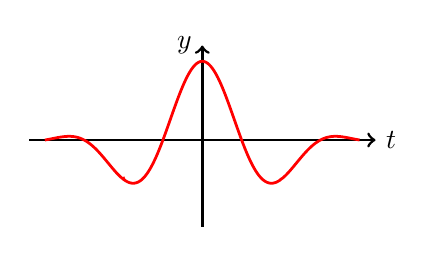
\begin{tikzpicture}[line width=1pt,domain=-2.2:2.2]
		\draw [->] (-2.2,0) -- (2.2,0) node[right] {$t$};
		\draw [->] (0,-1.1) -- (0,1.2) node[left] {$y$};
		%\draw plot[id=x] function{sin(3.1415926*x/8)*8/3.1415926/x*cos(3.1415926*x/8)/(1-(2*x/8)\^2)};
		\draw[domain=-2:2,samples=500,color=red] plot(\x,{sin(pi*\x r)/(pi*\x)*cos(pi*\x r)/(1-\x*\x)});
	\end{tikzpicture}
	\caption{升余弦函数$(\alpha=0.5)$}
	\label{Figure:ddcode:rcos}
\end{figure}

	基带传输信号$x(t)$为:
\begin{equation}
x(t)=\sum_{n=0}^{\infty}u[n]c(t-nT_s)
\end{equation}
其中,$T_s=GT_c$为码元宽度。通带传输信号$\widetilde{x}(t)$为:
\begin{equation}
\widetilde{x}(t)=Re\{x(t)e^{j2\pi f_ct}\}
\end{equation}
其中,$f_c$为载波频率。

	通带信号$\widetilde{x}(t)$的频谱由$\phi(t)$,$T_c$和$f_c$决定。如前所述,$\phi(t)$为均方根升余弦函数,设其滚降因子为$\alpha$,那么$\phi(t)$的周期(也就是扩频码宽度)为:\[ T_c=\frac{\alpha+1}{f_h-f_l} \]其中$f_h-f_l=B$为传输带宽。综上,系统的传输率为:
\begin{equation}
R_b=\frac{\log_2M}{G}\times\frac{B}{1+\alpha}
\end{equation}
其中$M$为PSK调制阶数,如:BPSK($M=2$),QPSK($M=4$)。



\subsection{DD-SS的接收机}
	在实际水声信道中,传输信号会经过不同的路径传输至接收端即所谓的多途传播。水声信道随时间空间亦会发生缓慢变化,文献\cite{俊英1992水下声信道}给出了多途时变信道的系统函数:
\begin{equation}
h(t)=\sum_{p=1}^{N_p}A_p(t)\delta(t-\tau_p(t))
\end{equation}
式中$A_p(t)$为每条多途的幅度,$\tau_p(t)$为每条多途的延时。如果假设信道变化缓慢,在第$m$个分析时间间隔内可以认为$A_p(t)$和$\tau_p(t)$是常数$A_p[m]$和$\tau_p[m]$,那么系统函数可以简化为:
\begin{equation}
h(t,m)=\sum_{p=1}^{N_p}A_p[m]\delta(t-\tau_p[m])
\end{equation}

	根据上述假设,接收信号$\widetilde{r}(t)$为:
\begin{equation}
	\widetilde{r}(t,m)=\sum_{p=1}^{N_p}A_p[m]\widetilde{x}(t-\tau_p[m])
\end{equation}
\begin{figure}[htbp]
	\centering
	\begin{tikzpicture}[auto, thick, node distance=3cm, >=triangle 45]
	\draw
	node [input,name=in] {}
	node [block,right of=in, xshift=-0.6cm] (mod) {\wuhao 载波解调}
	node [block, right of=mod] (encode) {\wuhao 匹配滤波}
	node [block, right of=encode] (DS) {\wuhao 峰值检测}
	node [block,right of=DS] (cm) {\wuhao 二阶差分检测}
	node [output, right of=cm,xshift=-0.6cm] (out){}
	node [below of=encode, yshift=1.5cm] (ct) {}
	;
	\draw [->] (in)--(mod);
	\draw [->] (mod)--node[anchor=south] {$r(t)]$}(encode);
	\draw [->] (encode) -- node[anchor=south] {$y(t)$} (DS);
	\draw [->] (DS) -- node[anchor=south] {$y[n]$} (cm);
	\draw [->] (cm) -- (out);
	\draw [->] (ct) -- node[anchor=east] {$c(t)$} (encode);
	
	%label
	\draw 
	node [above right] at (in) {$\widetilde{r}(t)$}
	node [above left] at (out) {$d[n]$};
	
	\end{tikzpicture}
	\caption{DD-SS接收机系统框图}
	\label{Figure::ddcode:ddssrecv}
\end{figure}

\subsubsection{接收机解扩频}
	经过载波解调后的信号$r(t)$可以表示为:
\begin{equation}
	r(t)=\sum_{p=1}^{N_p}A_p[m]e^{-2j\pi f_c\tau_p[m]}c(t-mT_s-\tau)u[m]
\end{equation}
式中$u[m]$表示接收到的第$m$个符号,并且忽略了码间串扰。文献\cite{liu2014long}假设延时$\tau_p[m]$是线性变化的,即:\[ \tau_p[m+1] -\tau_p[m]~=~\tau_p[m]-\tau_p[m-1] \]

	在$N_p$个多途中,通过同步技术能够找到能量最大的第$q$条多途。则解扩后的信号$y[m]$为:
\begin{equation}
	y[m]=\int_{D_{q,m}}^{}r(t)c(t-mT_s-\tau_p[m])
\end{equation}结合上述假设,可以得到\cite{liu2014long}:
\begin{equation}
	y[m]=A_q[m]e^{j2\pi f_c\tau_p[m]}u[m]
\end{equation}

\subsubsection{二阶差分检测}
	根据式(\ref{eq:ddcode:ddformula}),有:
\begin{equation}
\begin{split}
	d[n]&=\frac{v[n]}{v[n-1]} \\
	    &=\frac{u[n]}{u[n-1]}\times\frac{u[n-2]}{u[n-1]}
\end{split}
\end{equation}
类比上式并令$\phi_q[m]=-2\pi f_c \tau_q[m]$,进行如下变换:
\begin{equation}
\begin{split}
	z[m]=&\frac{y[m]}{y[m-1]}\times\frac{y[m-2]}{y[m-1]} \\
	=&\frac{A_q[m]e^{j\phi_q[m]} u[m]}{A_q[m-1]e^{j\phi_q[m-1]} u[m-1]} \times \frac{A_q[m-2]e^{j\phi_q[m-2]} u[m-2]}{A_q[m-1]e^{j\phi_q[m-1]} u[m-1]} \\
	=&\frac{A_q[m]A_q[m-2]}{A_q[m-1]A_q[m-1]}\times\frac{u[m]u[m-2]}{u[m-1]u[m-1]}\times e^{j\left[(\phi_q[m]-\phi_q[m-1]) - (\phi_q[m-1] - \phi_q[m-2])\right]}
\end{split}
\end{equation}
由$\tau_p[m+1] -\tau_p[m]~=~\tau_p[m]-\tau_p[m-1]$可得\[ (\phi_q[m]-\phi_q[m-1]) - (\phi_q[m-1] - \phi_q[m-2]) = 0 \]则:
\begin{equation}
\begin{split}
z[m]&=\frac{A_q[m]A_q[m-2]}{A_q[m-1]A_q[m-1]}\times\frac{u[m]u[m-2]}{u[m-1]u[m-1]} \\
    &=\frac{A_q[m]A_q[m-2]}{A_q[m-1]A_q[m-1]}d[m]
\end{split}
\end{equation}




		
	